\documentclass{article}

\usepackage[T1]{fontenc} % add special characters (e.g., umlaute)
\usepackage[utf8]{inputenc} % set utf-8 as default input encoding
\usepackage{ismir,amsmath,cite,url}
\usepackage{graphicx}
\usepackage{color}

\usepackage{lineno}
\linenumbers

% ------
\title{
Melody transcription via generative pre-training
%A fresh look at melody transcription
}

\threeauthors
  {First Author} {Affiliation1 \\ {\tt author1@ismir.edu}}
  {Second Author} {\bf Retain these fake authors in\\\bf submission to preserve the formatting}
  {Third Author} {Affiliation3 \\ {\tt author3@ismir.edu}}

% For the author list in the Creative Common license, please enter author names. 
% Please abbreviate the first names of authors and add 'and' between the second to last and last authors.
\def\authorname{F. Author, S. Author, and T. Author}

% Optional: To use hyperref, uncomment the following.
\usepackage[bookmarks=false,pdfauthor={\authorname},pdfsubject={\papersubject},hidelinks]{hyperref}
% Mind the bookmarks=false option; bookmarks are incompatible with ismir.sty.

\sloppy % please retain sloppy command for improved formatting

% My dependencies
\usepackage{booktabs}
\usepackage{cleveref}
\usepackage{amsfonts}
\usepackage{amssymb}

% My macros
\newcommand{\madmom}{\texttt{madmom}}
\newcommand{\mel}{Mel}
\newcommand{\mtthree}{MT3}
\newcommand{\jukebox}{Jukebox}
\newcommand{\hooktheory}{HookTheory}
\newcommand{\rwc}{RWC-MDB}
\newcommand{\sheetsage}{Sheet Sage}
\newcommand{\fone}{F1}

\newcommand{\cd}[1]{{\textcolor{blue}{[CD: #1]}}}
\newcommand{\jt}[1]{{\textcolor{magenta}{[JT: #1]}}}
\newcommand{\pl}[1]{\textcolor{red}{[PL: #1]}}
\newcommand{\todo}[1]{\textcolor{red}{[TODO: #1]}}
\newcommand\john[1]{\textcolor{magenta}{[JT: #1]}}

\begin{document}

\maketitle

\begin{abstract}
Melody 
%is among the most fundamental aspects 
is a fundamental aspect 
of 
%human 
music perception. 
%---even those without musical training can often recognize and reproduce melodies by ear. 
While even those without musical training can often recognize and reproduce melodies by ear, it remains an open challenge in MIR to transcribe an arbitrary recording of Western music into notes which constitute its melody. 
A key challenge in melody transcription is building methods which can handle broad audio containing any number of instrument ensembles and musical genres. 
To confront this challenge, we leverage recent advancements in generative modeling of broad music audio, thereby improving performance on melody transcription by up to $27$\% relative to conventional approaches. 
Another obstacle in melody transcription is a lack of training data---we collect, align, and release a new dataset consisting of $50$ hours of crowdsourced melody annotations for popular music. 
\todo{Mention that we trained a chord recognition model in the abstract?}
By pairing our new melody transcription approach with existing solutions for beat detection, key estimation, and chord recognition, 
we build the first system capable of transcribing human-readable lead sheets directly from music audio.\footnote{Sound examples: \url{https://dblblnd.github.io/ismir22} \\
Demo / dataset explorer: \url{https://colab.research.google.com/drive/1yzD3wRCjXkuSfDRUtt_daaGFitj5L88l}\label{sound_examples}}
\end{abstract}


\section{Introduction}\label{sec:introduction}

In the Western music canon (and especially in popular music), 
\emph{melody} is a defining characteristic of musical composition. 
Even those without formal musical training can often effortlessly recognize a melody within a complex mixture of sounds, 
a ubiquitous skill which forms a pillar of our collective musical experience. %experience. 
Because of the significance of melody to music perception, 
the ability to automatically \emph{transcribe} an arbitrary recording into 
%equal-tempered notes which constitute its melody 
its melody notes \john{awkward wording}
could enable numerous applications in 
% TODO: performance?
interaction~\cite{ryynanen2008accompaniment}, 
education~\cite{droe2006music}, 
informatics~\cite{bainbridge1999towards}, 
retrieval~\cite{ghias1995query}, 
source separation~\cite{ewert2014score},
and even generation~\cite{hawthorne2019enabling}.
Despite the numerous potential benefits, 
reliable melody transcription remains an open challenge in MIR.
%it remains an open challenge in MIR to transcribe an arbitrary recording into equal-tempered notes which constitute its melody.

% Why is it difficult?
The relative lack of progress on melody transcription is perhaps counterintuitive when compared to the considerable progress on seemingly more difficult tasks like piano transcription~\cite{sigtia2016end,hawthorne2017onsets}.
%and chord recognition~\cite{humphrey2012rethinking,boulanger2013audio}. 
This circumstance stems from two primary factors. 
First, unlike in piano transcription, melody transcription involves operating on \emph{broad} \john{diverse?} audio mixtures from arbitrary instrument ensembles and genres. 
% CHRIS: I think the following is indeed a big reason that melody transcription is hard, but it doesn't map cleanly onto any of our contributions
%Second, unlike in chord recognition, melody transcription involves isolating the notes from a single instrument voice (recognized to be the melodic voice) within the mixture. 
%Second, melody transcription involves not only detecting notes but also identifying which of those notes constitutes the melody, which may require modeling the nuances of human music perception. 
Second, little training data exists for melody transcription, which particularly impedes the deep learning approaches central to recent improvements in other areas of music transcription. 
% CHRIS: This maps cleanly onto our contributions (standardized evaluation and new datasets), but may be too snarky for paragraph 2
%Finally, we argue that a historical focus on the important but disparate task of melody \emph{extraction}---detecting the time-varying fundamental frequency of the melody as opposed to its discrete notes---has led to a lack of work on transcription and systemic issues in evaluation.

\begin{figure}
    \centering
    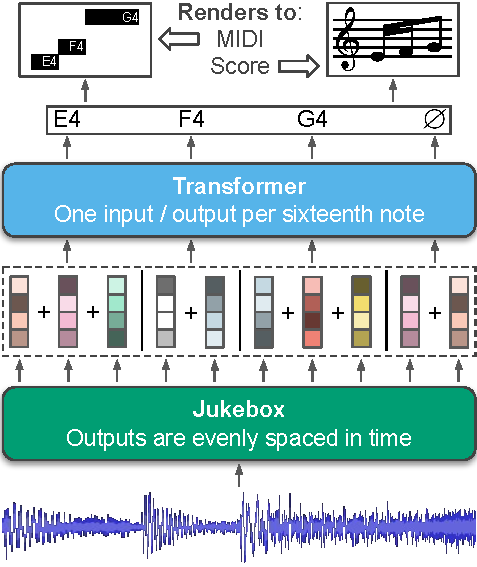
\includegraphics[width=8.1cm]{figs/fig1.pdf}
    \caption{
\john{Just aesthetics, but might want longer sequence of sheet music at the top of the figure (maybe need to change the audio to match)?} Our audio-to-score melody transcription approach involves 
(1)~extracting representations from Jukebox~\cite{dhariwal2020jukebox}, a generative model of music audio, 
(2)~averaging these representations across time to their nearest sixteenth note using \madmom~\cite{bock2016madmom,bock2016joint} for beat detection,
and
(3)~training a Transformer~\cite{vaswani2017attention} to detect melody note onsets (or rests) per sixteenth note.
}
 \label{fig:fig1}
\end{figure}

In order to overcome the challenge of transcribing broad audio, in this work we leverage representations from Jukebox~\cite{dhariwal2020jukebox}, a large-scale generative model of music audio pre-trained on $1$M songs~(\Cref{fig:fig1}). 
In~\cite{castellon2021calm}, Castellon~et~al.\ demonstrate that internal representations from Jukebox are useful for improving performance on a wide variety of MIR tasks. 
When used as input features to a Transformer~\cite{vaswani2017attention} model, representations from Jukebox outperform conventional spectrogram features used for melody transcription by 
% (RWC All) .744 vs .631 = 17.9%
% (Hookthr) .615 vs .514 = 19.6%
% (RWC Vox) .786 vs .621 = 26.6%
up to $27$\% (relative). 
% CHRIS: This can be cut for space
To the best of our knowledge, this is the first evidence that representations from generative models of audio are useful for time-varying MIR tasks like transcription, as opposed to the song-level tasks (e.g.~genre detection) examined in~\cite{castellon2021calm}. 

\john{Too many details here for introduction} To support this and future work on melody transcription, we collect and release a new dataset of crowdsourced melody annotations from the \hooktheory{} platform.\footnote{\url{https://www.hooktheory.com/theorytab}} 
This dataset contains $50$ hours of annotated melodies and harmonies (as chord names).  %and additionally contains chord labels.
%to aid chord recognition research. 
By training Transformer models on this new dataset using representations from Jukebox, we are able to improve overall performance on melody transcription by 
% 0.786 vs 0.462 = 70%
% 0.744 vs 0.420 = 77%
$77$\% 
relative to the strongest available baseline. 
While data from \hooktheory{} has been used previously for tasks like harmonization~\cite{chen2021surprisenet,yeh2021automatic}, chord recognition~\cite{jiang2019mirex}, and representation learning~\cite{jiang2020transformer}, making use of this platform for MIR is currently cumbersome and involves web scraping, reverse engineering a proprietary score format, and audio-to-score alignment. 
To ease this burden, we release all of the annotations in a simplified MIDI-like format under a Creative Commons license, with links and alignments to the audio on YouTube. 
We also release all code, models, and Docker containers needed for precisely reproducing all of our evaluations, facilitating comparison in future work even as some audio inevitably disappears from YouTube.\footnote{Released upon publication}

\john{Again too much detail} We also propose a new strategy for training transcription models in the presence of imprecise alignments. 
User annotations from \hooktheory{} have coarse alignments with the audio---users only provide the starting and ending timestamp of a segment. 
We use beat tracking to refine these alignments, but they are still not as precise as the flawless alignments found in other transcription datasets (e.g.,~piano transcription datasets captured using a Disklavier) which existing methods rely on. 
To address this, our approach involves aggregating input features (evenly spaced in \emph{time}) into proxy features which represent individual sixteenth notes (evenly spaced in \emph{beats}), 
which effectively smooths over alignment jitter. 
This approach has a secondary benefit of trivializing the process of converting output from the transcription model into a human-readable score format. %which is simpler for musicians to interpret compared to MIDI.

\begin{figure*}
    \centering
    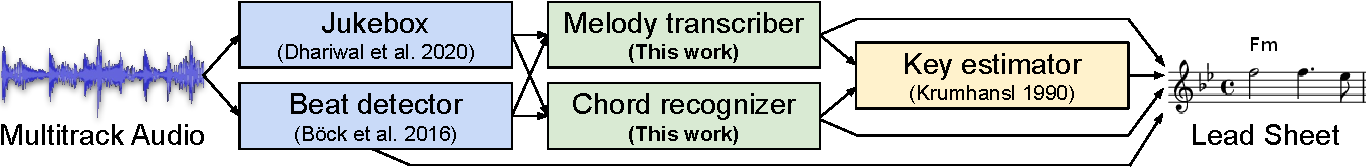
\includegraphics[width=\linewidth]{figs/sheet_sage.pdf}
    \caption{
    % TODO: Clean this up. YouTube as input
    Inference procedure for Sheet Sage, our proposed system which transcribes any Western music audio into lead sheets (scores which depict melody as notes and harmony as chord names). The blue, green, and yellow boxes respectively take audio, features, and symbolic music data as input. Green boxes are modules that we built as part of this work---both are Transformers~\cite{vaswani2017attention} trained on their respective tasks using audio features from Jukebox~\cite{dhariwal2020jukebox} and data from \hooktheory~\cite{hooktheory}.}
    \label{fig:sheet_sage}
\end{figure*}

\john{Again, detail} Finally, enabled by our state-of-the-art melody transcription approach, we present \emph{\sheetsage}, a system capable of automatically transcribing Western music audio into \emph{lead sheets}. 
A lead sheet is a human-readable musical score depicting a song's melody as notes on a staff and its harmony as chord names. 
The combination of melody and harmony represents the essence of a piece of Western music, and as such, lead sheets are commonly used by experts to easily perform recognizable renditions of existing pieces. 
As part of \sheetsage, we additionally train a Transformer-based chord recognition model on \hooktheory{} data using input features from Jukebox. 
To produce lead sheets, we pair this chord recognition model with our best melody transcription model, beat detections from \madmom~\cite{bock2016madmom,bock2016joint}, key estimations from Melisma~\cite{krumhansl1990cognitive,temperley1999key,sleator2001melisma}, and engraving with LilyPond~\cite{nienhuys2003lilypond}~(\Cref{fig:sheet_sage}). 
By automatically transcribing music audio into lead sheets, our work helps reduce the gap between human perception and machine understanding of Western music.

\john{Suggestion: condense the last 3 paragraphs of the intro into a bulleted list of contributions. Move all the details later into the paper}

\section{Related work}

Melody transcription is often cast as a melody \emph{extraction} task, which requires us to annotate an audio recording with a time-varying, continuous fundamental frequency (F0) estimate \cite{goto2004real}. Melody extraction has been popularized by annual results of the MIREX Audio Melody Extraction tasks \cite{downie2014ten}, garnering significant interest from the MIR community over the last two decades \cite{salamon2014melody,rao2022melody}. In contrast, our work is concerned with transcription to human-readable \emph{lead sheets}: this task requires us to indicate the positions of notes within a metrical structure, belonging to discrete pitch classes.

Lead-sheet melody transcription has received considerably less attention. Poliner et. al. observed in 2007 that ``an attempt was made to evaluate the lead voice transcription at the lowest level of abstraction [melody extraction], and as such, the concept of segmenting the fundamental frequency predictions into notes has been largely omitted from consideration'' \cite{poliner2007melody}. This omission largely remains true today. To the best of our knowledge, there have been only three efforts to transcribe melodies to lead sheets since 2007 \cite{ryynanen2008automatic,weil2009automatic,laaksonen2014automaticO}; we compare our melody transcription results with \cite{ryynanen2008automatic} in \cref{sec:experiments}.

Polyphonic music transcription has received substantial attention, with its own MIREX task (Multiple Fundamental F0 Estimation) and a growing collection of supervised training data resources \cite{benetos2013automatic,thickstun2017learning,hawthorne2019enabling,manilow2019cutting}. Like melody transcription, polyphonic transcription is typically formalized as a low-level \emph{frame-based} transcription task, which requires us to annotate an audio recording with a time-aligned piano roll. Like melody extraction, this task does not result in a human-readable lead sheet or score. Nevertheless, the similarity of the polyphonic and melody transcription problems, together with recent progress towards polyphonic transcription, motivate us to consider whether representations learned by a polyphonic music transcription system, MT3 \cite{gardner2021mt3}, are useful for melody transcription.

% TODO

\section{Task definition}

\begin{figure}
    \centering
    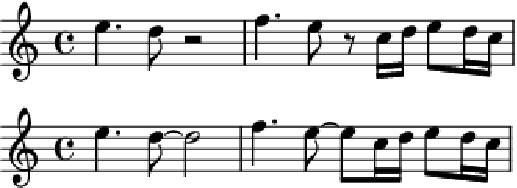
\includegraphics[width=8.1cm]{figs/heuristic_offsets.pdf}
    \caption{
The same note onsets engraved with ground truth~(top) vs. heuristic~(bottom) offsets. 
We argue that onset prediction suffices for producing melody transcriptions that are both recognizable and readable. 
}
 \label{fig:heuristic_offsets}
\end{figure}

\john{You may want to lead here with two definitions: the definition of \emph{melody} (implicitly defined by labels) and the definition of \emph{melody transcription} (in contrast to melody extraction)}

We examine melody transcription, defined here as the task of converting music audio into a \emph{monophonic} (non-overlapping) sequence of \emph{notes} which constitute its melody. 
A note canonically consists of an onset time, a musical pitch, and an offset time, though here (and as in~\cite{laaksonen2014automatic}) we disregard offsets for several reasons. 
First, accuracy of onsets has been found to be far more important to human perception of transcription quality than accuracy of offsets~\cite{ycart2020investigating}. 
Second, in our dataset (which represents a crowdsourced proxy in lieu of a precise definition of melody), a heuristically-determined offset is identical to the ground truth offset for $89\%$ of notes.\footnote{The heuristic we adopt sets the offset of one note equal to the onset of the next, i.e., it assumes the melody is legato.}
Finally, we argue intuitively that onsets and pitches suffice for both recognizing and reading melodies---see~\Cref{fig:heuristic_offsets} for an example. 

Formally, \john{want me to make this more formal? ;)} the task of melody transcription is to convert music audio $\bm{a}$, sampled at rate $f_s$, into a list of notes $\bm{y}$, where a note $y_i$ is a pair of onset time $t_i$ and musical pitch $n_i$. Hence, 
\begin{align*}
    \bm{a} &= a_1, \ldots, a_S, \text{where}~S = Tf_s \\
    \bm{y} &= y_1, \ldots, y_N, \text{where}~y_i = (t_i, n_i).
        %&&t_i \leq T, \text{and} n_i \in \{\text{A0}, \ldots, \text{C8}\}
\end{align*}
To handle the high dimensionality of audio, transcription algorithms typically extract features $\bm{X}$ (a matrix) from audio, which are sampled at $f_k \ll f_s$:
\begin{align*}
    \text{Extract}(\bm{a}) = \bm{X} = \bm{x}_1, \ldots, \bm{x}_M, \\ 
    \text{where}~M = Tf_k~\text{and}~\bm{x}_i \in \mathbb{R}^d.
\end{align*}
Hence, in practice, our goal is to build a transcription method 
$f : \bm{X} \mapsto \bm{y}$.
% $f$ which maps features $\bm{X}$ to notes $\bm{y}$. 

\subsection{Evaluation}
\label{sec:eval}

\john{Leading with an MIR implementation of F1 is a little confusing, especially since it is not typically applied to this task (you are defining the task, right?)}
To evaluate a melody transcription method $f$, 
we incorporate a standard approach~\cite{raffel2014eval} for computing an \fone{} score between reference $\bm{y}$ and estimate $f(\bm{X})$. 
This approach---shown in~\cite{ycart2020investigating} to correlate with human perception---scores estimates by aligning their onsets to the reference onsets with $50$ms of tolerance, and then computes a standard \fone{} score, where an estimated note is treated as correct if it is the same pitch as the matched reference:
\begin{equation*}
    \text{Score} : f(\bm{X}), y \mapsto [0, 1].
\end{equation*}

\john{This adjustment seems to be needed because of the nature of the annotations (next section) but it's pretty confusing introducing it before that discussion}
In other transcription settings, evaluation conventionally requires that estimates match the octave of the reference. 
In melody transcription, where transcriptions are prone to be performed on different instruments or by vocalists with different ranges, predicting the correct octave is less critical for downstream use. 
Previous evaluations for melody extraction gave full credit for estimates with the right pitch class (see~\cite{poliner2007melody} for a summary), however we argue that \emph{relative} octave information is important for transcription accuracy. 
Hence, we modify the evaluation criteria to allow models to achieve a perfect score if they produce the correct notes but are off by a fixed octave shift:
\begin{equation*}
    \max_{i \in \mathbb{Z}} \text{Score}(\text{OctaveShift}(f(\bm{X}), i), \mathbf{y}).
\end{equation*}

\section{Dataset overview}
\label{sec:dataset}

\begin{figure}
    \centering
    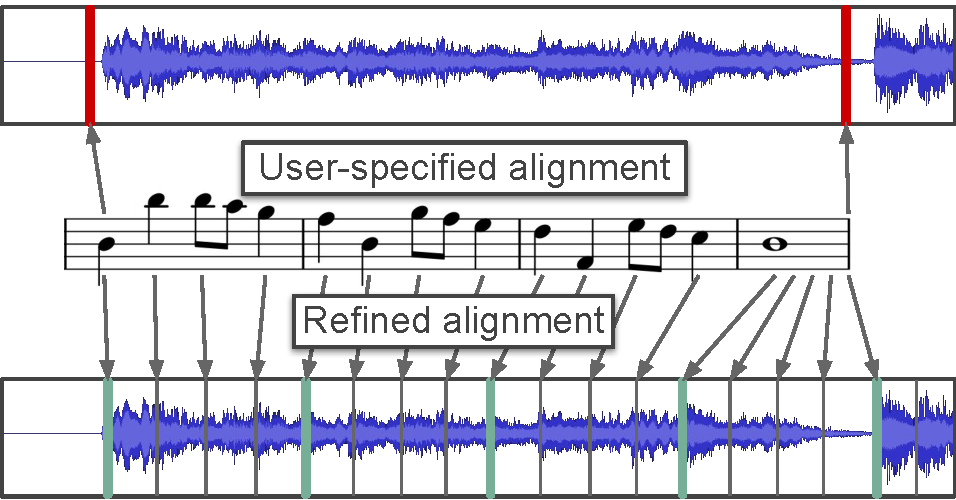
\includegraphics[width=8.1cm]{figs/alignment.pdf}
    \caption{We refine coarse, user-specified alignments from \hooktheory{} by using beat tracking. The first segment beat is mapped to the detected downbeat nearest to the user-specified starting timestamp, and remaining beats are mapped to subsequent detected beats.}
 \label{fig:alignment}
\end{figure}

We collect and release a dataset of crowdsourced melody and chord annotations from \hooktheory{}. 
The dataset comprises annotations for $22$k segments of $13$k unique recordings---together, these segments comprise $50$ hours of labeled audio. 
The audio content covers a wide range of genres---there is a skew towards pop and rock but many other genres are represented including EDM, jazz, and even classical. 
We create an artist-stratified $8$:$1$:$1$ split of the dataset for training, validation, and testing.

\hooktheory{} users annotate the audio in a proprietary ``functional'' format, i.e., one which uses scale degrees and roman numerals relative to a key signature instead of absolute notes and chord names. 
Absolute labels are used by the vast majority of transcription work---hence, we convert this proprietary functional format into a simple absolute one. 
Note that users annotate melodies with only relative octave information, i.e.,~intervals between melody notes should be accurate, but the absolute octave of the melody may be incorrect relative to the recording.

\subsection{Alignment}

With the release of this dataset, we also make an effort to improve the alignments between the annotations and the audio. 
By default, users provide only a coarse audio alignment, specifying the starting and ending timestamps of the annotated segment. 
These alignments are overall poor---the starting/ending timestamps are often sloppy, and any tempo fluctuations within a segment will further jeopardize the alignment.

We use the beat and downbeat detection algorithm from \madmom{}~\cite{bock2016joint,bock2016madmom} to refine these alignments. 
Our approach aligns the first beat of the segment to the detected downbeat which is nearest to the user-specified starting timestamp. 
Then, we align the remaining beats to the subsequent consecutive detected beats (see~\Cref{fig:alignment} for an example). 
This provides a beat-level alignment for the entire segment, and we use linear interpolation for fractional beat subdivisions. 
In an informal listening test, this produces an excellent alignment in around $95\%$ of cases, where the primary failure mode in the remaining $5\%$ occurs when \madmom{} detects the wrong beat as the downbeat. 
We use these refined alignments for training and evaluation, accepting the glitched alignments as noise in the dataset.

\section{Methods}

As in state-of-the-art methodology for other areas of transcription~\cite{hawthorne2021sequence}, 
our approach to melody transcription involves training Transformer~\cite{vaswani2017attention} models to predict notes from audio features. 
However, our approach differs in two distinct ways to address to the challenges unique to melody transcription.
First, because melody transcription involves operating on broad audio, we leverage representations from pre-trained models as drop-in replacements for the handcrafted spectrogram features used as inputs to other transcription systems. 
Secondly, because alignments in our dataset are approximate, we propose a new strategy for training transcription models under such conditions.

\subsection{Pre-trained representations}
\label{sec:representations}

We explore representations from two different pre-trained models for use as input features to transcription models.
In~\cite{castellon2021calm}, Castellon~et~al.\ demonstrate that representations from \jukebox---a generative model of music audio pre-trained on $1$M songs---constitute general purpose features for MIR tasks, though notably they do not verify this claim for transcription. 
We adopt their approach to extract features from \jukebox{} ($f_k \approx 345$ Hz, $d = 4800$), however we pull representations from a deeper layer of \jukebox{} ($54$ vs. $36$), which Castellon~et~al.\ found to be more effective for note-aware tasks like key estimation. 

We also explore features from \mtthree~\cite{gardner2021mt3}, an encoder-decoder transcription model pre-trained on a multitude of different transcription tasks (though not melody transcription). 
For this model, we use the output of the encoder ($f_k = 125$ Hz, $d = 512$) as our feature representation. 
The two models have different trade-offs with respect to our setting: \jukebox{} was trained on audio similar to that found in our dataset but explores a different task (generative modeling), whereas \mtthree{} is pre-trained on transcription but for different audio domains. 

\subsection{Beat pooling}

% Alignment
Despite our best efforts, the refined alignments in \hooktheory{} are still imprecise when compared to those found in datasets used by piano transcription methods. 
In initial experiments, we found that naively adopting methods designed for piano transcription~\cite{hawthorne2017onsets,hawthorne2021sequence} resulted in poor performance on our dataset and task.\footnote{Additionally, training models with an alignment-free approach~\cite{graves2006connectionist} also resulted in poor performance.} 
Hence, we designed a new approach for training models in the presence of approximate alignments. 

Our approach works by averaging all of the feature vectors (equally spaced in time) that are nearest to a particular sixteenth note into a single vector which acts as a proxy feature for that sixteenth note. 
For example, if a recording has a tempo of $120$ beats per minute, a sixteenth note represents $125$ ms of time, which would mean averaging across around $43$ feature vectors from \jukebox{} ($f_k \approx 345$ Hz). 
The intuition is that, while our beat tracked alignments may not be able to identify precisely where the ground truth onset occurs in these $43$ frames, we can be reasonably confident that it occurs \emph{somewhere} within them, and thus that information will be incorporated into the feature vector.
We refer to this strategy as \emph{beat pooling}.

\todo{John, I could use your eyeballs / refinement on this. One question is whether or not the 1-based indexing for beats makes this super confusing. Feel free to ask for clarification on anything}
Formally, for a segment of length $T$ seconds and $B$ beats, and an alignment function $a: [0, T] \mapsto [1, B]$, beat pooling yields a matrix $\hat{\bm{X}} = \hat{\bm{x}}_1, \ldots, \hat{\bm{x}}_{4B}$, where $\hat{\bm{x}}_i \in \mathbb{R}^d$, and
\begin{gather*}
\bm{\hat{x}}_i = \frac{1}{r_i - l_i} \sum_{j = l_i}^{r_i - 1} \bm{x}_j, \text{where} \\
l_i = \left\lfloor a \left(\frac{2i + 5}{8} \right) \cdot f_k \right\rfloor, \text{and}~
r_i = \left\lfloor a \left(\frac{2i + 7}{8} \right) \cdot f_k \right\rfloor.
\end{gather*}

\subsection{Training}

The output of our beat pooling approach ($\hat{\bm{X}}$) represents a sequence of features where a timestep is a sixteenth note, and constitutes the input to the transcription model we will train. 
Analogously, we also construct a sequence containing labels for each sixteenth note $\hat{\bm{y}} \in \mathbb{V}^{4B}$, where 
$\mathbb{V} = \{\varnothing, \text{A0}, \ldots, \text{C8}\}$.\footnote{This requires quantizing labels to the nearest sixteenth note. In practice, less than $1\%$ of notes are affected by this quantization, and $99\%$ of segments contain no affected notes.} 
This sequence indicates for each sixteenth note whether or not an onset occurs ($\varnothing$ if not, note name if so). 
Then, we can formulate melody transcription as an aligned sequence-to-sequence modeling problem and train models of the form $f_{\theta} : \mathbb{R}^{4B \times d} \mapsto \mathbb{R}^{4B \times |\mathbb{V}|}$ using a standard cross entropy loss. 

An additional challenge is that octave information is often incorrect in our dataset (see \Cref{sec:dataset}). 
Hence, we construct an octave-tolerant loss function by octave shifting the labels and backpropagating on whichever shift minimizes the loss:
\begin{equation*}
\operatorname*{min}_{\sigma \in \{-\alpha, \ldots, \alpha\}} \sum_{i=1}^{4B} \text{CrossEntropy}(f_{\theta}(\bm{\hat{X}})_i, \text{OctaveShift}(\hat{\bm{y}}_i, \sigma)). 
\end{equation*}
Here, $\alpha$ is an integer determining the number of possible shifts, and $\alpha = 0$ constitutes the standard cross entropy loss. 
In practice, we found $\alpha = 2$ produced the best results, while $\alpha > 3$ resulted in unstable training.

\section{Experiments}
\label{sec:experiments}

Here we describe our experimental protocol for training melody transcription models on the \hooktheory{} dataset. 
The purpose of these experiments is two-fold. 
First, we compare representations from different pre-trained models to handcrafted spectrogram baselines, to determine if these representations are helpful for the task of melody transcription.  
Second, we compare our trained models holistically to other melody transcription baselines. 

All transcription models are encoder-only Transformers with the default hyperparameters from~\cite{vaswani2017attention}, 
except that we reduce the number of layers from $6$ to $4$ to allow models to be trained on GPUs with $12$GB of memory. 
During training, we select random slices from the annotated segments of up to $96$ beats or $24$ seconds in length (whichever is shorter). 
We train using our proposed octave-invariant loss function with $\alpha = 2$. 
We perform early stopping based on max \fone{} score across thresholds on the validation set, using the best validation threshold during testing. 
All models converge within $15$k steps which takes about a day on a single K40 GPU (features are separately precomputed). 

\subsection{Comparing input features}
\label{sec:exp1}

\begin{table}[t]
    \centering
    \begin{tabular}{lcc}
\toprule
Features & $d$ & Onset \fone{} \\
\midrule
\mel{} & $229$ & $0.514$ \\
\mtthree{} & $512$ & $0.550$ \\
\jukebox{} & $4800$ & $0.615$ \\
\mel{}, \mtthree{} & $741$ & $0.548$ \\
\mel{}, \jukebox{} & $5029$ & $0.617$ \\
\mtthree{}, \jukebox{} & $5312$ & $0.622$ \\
\mel{}, \mtthree{}, \jukebox{} & $5541$ & $\mathbf{0.623}$ \\
\bottomrule
    \end{tabular}
    \caption{\hooktheory{} test set performance of different combinations of representations (when passed as input to train a Transformer). Different representations do contain complimentary information---combining all three yields highest performance---but Jukebox on its own is competitive with all combinations.}
    \label{tab:hooktheory_test}
\end{table}

We compare representations from \jukebox~\cite{dhariwal2020jukebox} and \mtthree~\cite{gardner2021mt3} (see~\Cref{sec:representations}) to handcrafted spectrogram features which constitute the conventional inputs to existing transcription methods. 
Specifically, we compare to log-amplitude Mel spectrograms using the formulation from~\cite{hawthorne2017onsets} ($f_k \approx 31$, $d = 229$). 
Because features may contain complimentary information, we also experiment with all combinations of these three features. 
Note that our beat pooling strategy makes it trivial to combine these features (by concatenation) despite their differing rates. 
In~\Cref{tab:hooktheory_test}, we report \fone{} (as described in~\Cref{sec:eval}) on the \hooktheory{} test set for all input features.

Overall, using representations from \jukebox{} as input features results in stronger melody transcription performance than using either representations from \mtthree{} or conventional handcrafted features. 
Representations from either \mtthree{} or \jukebox{} outperform conventional handcrafted features, 
implying that either pre-training strategy is helpful for melody transcription. 
Note that these two pre-training approaches are compared holistically---these models differ on several axes (number of parameters, number of dimensions, pre-training data size and semantics, pre-training task), 
and thus it is impossible to disentangle the individual contributions of these different factors without retraining the models. 
%We also note that fine tuning these models would likely be more effective than using their representations as input features\cite{???}

Qualitatively speaking, there is a noticeable difference in performance across the three different input features which correlates with quantitative performance (see~\cref{sound_examples}). 
Using representations from \jukebox{} tends to result in fewer wrong notes than the other features, and substantially reduces the number of egregiously wrong notes (e.g.,~notes outside of the key signature). 
These representations also improve accuracy of nuanced rhythmic patterns in comparison to the other two. 
Moreover, using handcrafted features will often result in several onsets for a longer sustained melody note---in contrast, using representations from \jukebox{} appears to more consistently avoid repeat onsets for sustained notes. 

Some representations also appear to complement one another to a degree---the strongest performance overall is obtained by combining all three features. 
Combining \mtthree{} and \jukebox{} does improve performance over \jukebox{} alone, though only by a marginal amount. 
Using both pre-trained models is impractical considering the marginal returns---it almost doubles the overall transcription runtime, and the models also have incompatible software dependencies. 
Hence, in the remainder of this paper we focus on models trained on individual input features.
%Combining handcrafted features w/ either pre-trained approach has little effect on performance. 

\subsection{Comparison to melody transcription baselines}

\begin{table}[t]
    \centering
    \begin{tabular}{lcc}
\toprule
 & Onset \fone{} & Onset \fone{} \\
Approach & \emph{Vox Only} & \emph{All} \\
\midrule
MT3 Zero-shot~\cite{gardner2021mt3} & $0.085$ & $0.133$ \\
Melodia~\cite{salamon2014melody} + Segmentation & $0.268$ & $0.201$ \\
DSP + HMM~\cite{ryynanen2006transcription,ryynanen2008automatic} & $0.381$ & $0.420$ \\
Spleeter~\cite{hennequin2020spleeter} + Tony~\cite{mauch2015computer} & $0.462$ & $0.341$ \\
\midrule
\mel{} + Transformer & $0.621$ & $0.631$ \\
\mtthree{} + Transformer & $0.659$ & $0.701$ \\
\jukebox{} + Transformer & $\mathbf{0.786}$ & $\mathbf{0.744}$ \\
\bottomrule
    \end{tabular}
    \caption{Performance of different approaches on a small subset of \rwc~\cite{goto2002rwc,goto2003rwc,goto2004development}. The bottom three approaches were trained on the \hooktheory{} dataset as part of this work. We compute performance on both vocals and all melody instruments for fair comparison to baselines designed for vocal transcription.}
    \label{tab:rwc_ryy}
\end{table}

We compare holistic performance of our proposed melody transcription approach to several baselines. 
A handful of earlier works investigate melody transcription~\cite{ryynanen2008automatic,weil2009automatic,laaksonen2014automatic}, however all of these methods are sophisticated expert systems which would be extraordinarily difficult to reproduce, and none of these papers provide code. 
Fortunately,~\cite{ryynanen2008automatic} provide melody transcriptions for a small subset of $10$ songs from RWC-MDB~\cite{goto2002rwc,goto2003rwc,goto2004development}, 
which we adopt as an evaluation set for our holistic comparisons.

In addition to~\cite{ryynanen2008accompaniment}, we also compare to a baseline which applies a note segmentation heuristic to a melody extraction algorithm~\cite{salamon2014melody}. 
While \mtthree{} was not trained on melody transcription, it was trained on some tasks which involve vocal transcription---we examine zero-shot performance of this model as a baseline. 
Finally, because the vocals often carry the melody in popular music, we compare to a baseline of running the Tony~\cite{mauch2015computer} monophonic instrument transcription software on source-separated vocals isolated with Spleeter~\cite{hennequin2020spleeter}. 
Because this approach will only work for vocals, we also separately report performance on a subset of our evaluation set where the vocals represent the melody. 
It is worth noting that vocal isolation and transcription may be another promising path towards melody transcription, 
as it is unclear the extent to which transcribing non-vocal melodies is essential for downstream applications.
Scores for all methods and baselines appear in~\Cref{tab:rwc_ryy}. 

Overall, our approach to training Transformers with features from \jukebox{} significantly outperforms the strongest baseline in both the vocals only and unrestricted settings (\todo{p values}). 
Qualitatively speaking, ... \todo{}.
% Make sure to discuss both the good and the bad!
Performance of our approach using different input representations is consistent with evaluation results on the \hooktheory{} test set. 

\section{Sheet Sage}

\section{Conclusion}


\bibliography{main}

\end{document}

